\documentclass[11pt]{article}
\usepackage[a4paper,margin=1in]{geometry}
\usepackage{amsmath,amssymb,amsthm,mathtools}
\usepackage{graphicx}
\usepackage{microtype}
\usepackage{enumitem}
\usepackage{xcolor}
\usepackage[hidelinks]{hyperref}

\newtheorem{theorem}{Theorem}
\newtheorem{lemma}{Lemma}
\newcommand{\K}{\mathbb K}
\newcommand{\pair}[2]{\langle #1,#2\rangle}
\newcommand{\id}{\operatorname{id}}
\newcommand{\linspan}{\operatorname{span}}

\title{The Banach-Orthogonality Decomposition\\Without Reflexivity}
\author{Candidate full solution packet for arXiv:1610.00423, Problem 5}
\date{11 August 2026}

\begin{document}
\maketitle

\begin{center}
\fbox{\parbox{0.92\textwidth}{\textbf{Status.} Candidate full solution, likely valid, pending human review. The theorem below removes the reflexivity hypothesis from Sadr's characterization.}}
\end{center}

\section{Source and exact question}

Maysam Maysami Sadr, \emph{Decomposition of functions between Banach spaces in the orthogonality equation}, arXiv:1610.00423v2, subsequently published in \emph{Aequationes Mathematicae} 91 (2017), 739--743 \cite{Sadr}. The question is Problem 5 on source PDF page 4:

\begin{quote}
``Characterize the solutions of (1) in the case that $F$ is not reflexive.''
\end{quote}

Here equation (1) is
\begin{equation}\label{eq:orthogonality}
  \pair{f(x)}{g(\alpha)}=\pair{x}{\alpha}
  \qquad (x\in E,\ \alpha\in E^*),
\end{equation}
where $E,F$ are Banach spaces, $f:E\to F$ and $g:E^*\to F^*$ are arbitrary maps, and the brackets are the canonical duality pairings.

\begin{figure}[ht]
  \centering
  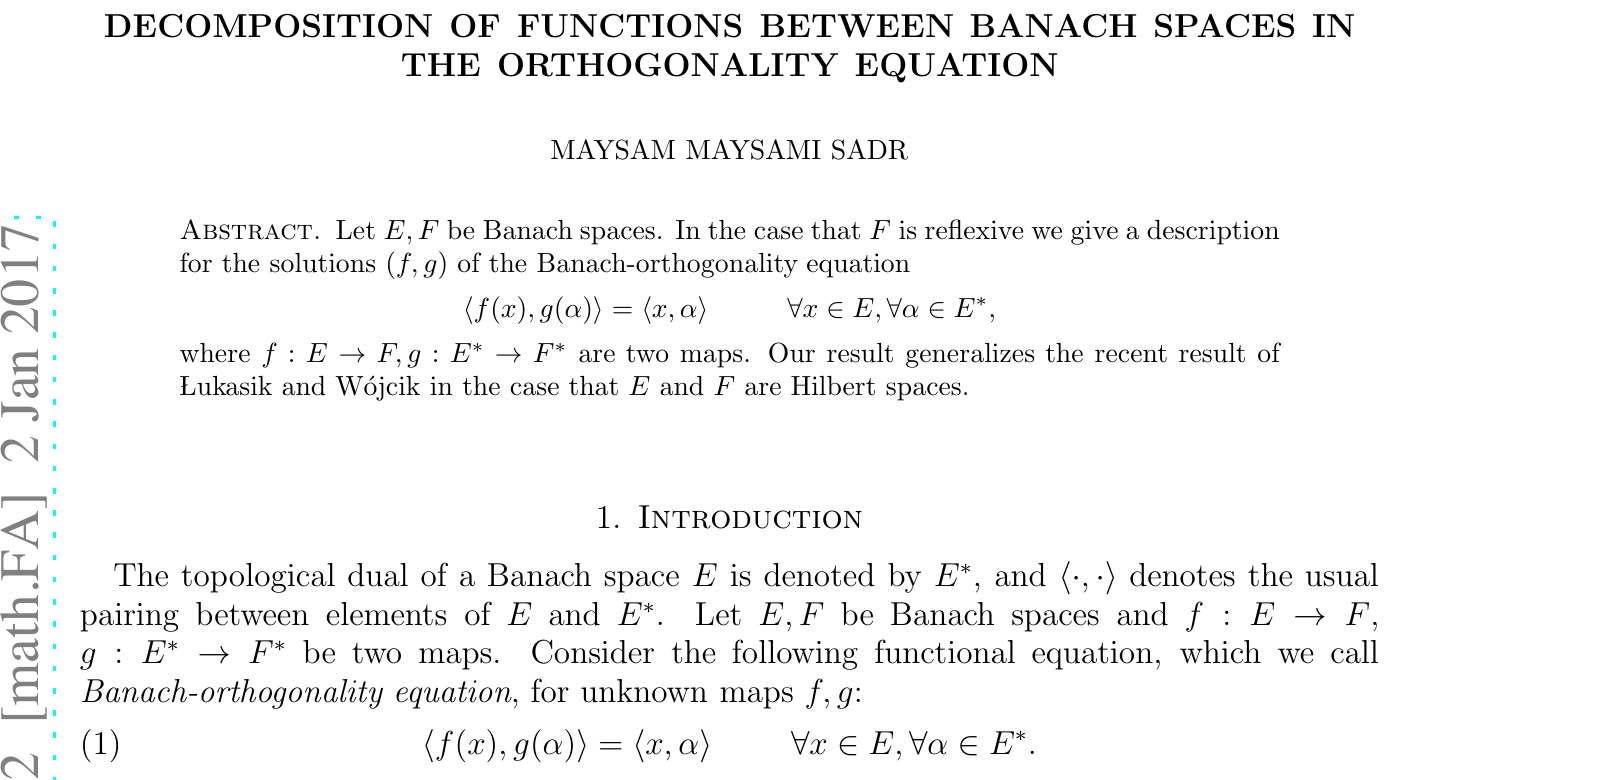
\includegraphics[width=\textwidth]{figures/equation_context_crop.png}
  \caption{The source's definition of equation (1), source PDF page 1.}
\end{figure}

\begin{figure}[ht]
  \centering
  
\includegraphics[width=\textwidth]{figures/open_problem_crop.png}
  \caption{Problem 5 in the source, PDF page 4.}
\end{figure}

\section{Answer and proof intuition}

The answer is that the characterization already proved in the source for reflexive $F$ remains valid \emph{verbatim} for arbitrary $F$.

The source uses reflexivity to identify a norm-closed subspace of $L^*$ with a double annihilator and thereby obtain norm density in a quotient dual. Norm density is stronger than necessary. If
\[
  M=Q(E^*)^\perp,
\]
then the induced family of functionals on $L/M$ is automatically \emph{total}: a coset annihilated by all of them has a representative in $M$, hence is zero. Totality alone detects additivity and homogeneity of the quotient-valued part of $f$. It also detects limits, so the closed graph theorem supplies boundedness. The original lower bound and density argument then make that quotient map an isomorphism. Thus the equation itself upgrades the initially total dual family to the entire quotient dual, with no reflexivity assumption.

\section{Reflexivity-free characterization}

All Banach spaces below are over the same scalar field $\K\in\{\mathbb R,\mathbb C\}$. If $M$ is a closed subspace of $L$, let
\[
  P:L\longrightarrow L/M
\]
be the quotient map and let
\[
  J:(L/M)^*\longrightarrow L^*,\qquad J\eta=\eta\circ P,
\]
be the canonical isometric injection. If $L$ is a closed subspace of $F$, let $R:F^*\to L^*$ be restriction.

\begin{theorem}[Answer to Problem 5]\label{thm:main}
Let $E$ and $F$ be arbitrary Banach spaces; no reflexivity is assumed. For arbitrary maps $f:E\to F$ and $g:E^*\to F^*$, equation \eqref{eq:orthogonality} holds if and only if there exist
\begin{enumerate}[label=\textup{(\roman*)}]
  \item closed linear subspaces $M\subseteq L\subseteq F$;
  \item a bounded linear isomorphism $A:E\to L/M$;
  \item a not necessarily linear right inverse $\varphi:L/M\to L$ of $P$;
  \item a not necessarily linear right inverse $\psi:L^*\to F^*$ of $R$;
\end{enumerate}
such that
\begin{equation}\label{eq:decomp}
  f=\varphi A,
  \qquad
  g=\psi J(A^*)^{-1}.
\end{equation}
\end{theorem}

\begin{proof}
The sufficiency of the representation is immediate but is included for completeness. If \eqref{eq:decomp} holds, then, for $x\in E$ and $\alpha\in E^*$,
\begin{align*}
 \pair{f(x)}{g(\alpha)}
 &=\pair{\varphi Ax}{\psi J(A^*)^{-1}\alpha}
  =\pair{\varphi Ax}{J(A^*)^{-1}\alpha}\\
 &=\pair{P\varphi Ax}{(A^*)^{-1}\alpha}
  =\pair{Ax}{(A^*)^{-1}\alpha}
  =\pair{x}{\alpha}.
\end{align*}
The second equality uses $R\psi=\id_{L^*}$ and the third uses the definition of $J$.

Conversely, suppose that \eqref{eq:orthogonality} holds. Put
\[
  L:=\overline{\linspan f(E)}\subseteq F,
  \qquad Q:=Rg:E^*\longrightarrow L^*.
\]
We first record that $Q$ is bounded linear. Indeed, for $\alpha,\beta\in E^*$ and $c\in\K$, the functionals
\[
 Q(\alpha+\beta)-Q\alpha-Q\beta,
 \qquad Q(c\alpha)-cQ\alpha
\]
vanish on $f(E)$ by \eqref{eq:orthogonality}; hence they vanish on the dense linear span of $f(E)$ and are zero on $L$. Thus $Q$ is linear. If $\alpha_n\to\alpha$ in $E^*$ and $Q\alpha_n\to\lambda$ in $L^*$, then for every $x\in E$,
\[
 \pair{f(x)}{\lambda}
 =\lim_n\pair{f(x)}{Q\alpha_n}
 =\lim_n\pair{x}{\alpha_n}
 =\pair{x}{\alpha}
 =\pair{f(x)}{Q\alpha}.
\]
Density again gives $\lambda=Q\alpha$. The graph of $Q$ is closed, so the closed graph theorem makes $Q$ bounded.

Define
\[
  M:=Q(E^*)^\perp
  =\{\ell\in L:\pair{\ell}{Q\alpha}=0\text{ for every }\alpha\in E^*\}.
\]
Then $M$ is a closed linear subspace of $L$. Each $Q\alpha$ annihilates $M$, so there is a unique bounded linear operator
\[
  \widehat Q:E^*\longrightarrow (L/M)^*
  \quad\text{with}\quad J\widehat Q=Q.
\]
The range $\widehat Q(E^*)$ is total on $L/M$. In fact, if $\ell+M\in L/M$ and
\[
  \pair{\ell+M}{\widehat Q\alpha}=0
  \quad\text{for every }\alpha\in E^*,
\]
then $\pair{\ell}{Q\alpha}=0$ for every $\alpha$, so $\ell\in M$ and $\ell+M=0$.

Let
\[
  B:=Pf:E\longrightarrow L/M.
\]
It need not initially be assumed linear. The original equation becomes
\begin{equation}\label{eq:BQ}
  \pair{Bx}{\widehat Q\alpha}=\pair{x}{\alpha}
  \qquad(x\in E,\ \alpha\in E^*).
\end{equation}
For $x,y\in E$, the vector $B(x+y)-Bx-By$ is annihilated by every member of $\widehat Q(E^*)$, by \eqref{eq:BQ}. Totality therefore makes it zero. The same argument applied to $B(cx)-cBx$ proves homogeneity. Hence $B$ is linear.

The same totality argument gives a closed graph. Namely, if $x_n\to x$ in $E$ and $Bx_n\to z$ in $L/M$, then for every $\alpha\in E^*$,
\[
 \pair{z}{\widehat Q\alpha}
 =\lim_n\pair{Bx_n}{\widehat Q\alpha}
 =\lim_n\pair{x_n}{\alpha}
 =\pair{x}{\alpha}
 =\pair{Bx}{\widehat Q\alpha}.
\]
Thus $z=Bx$, and the closed graph theorem shows that $B$ is bounded.

For each nonzero $x\in E$, Hahn--Banach provides $\alpha\in E^*$ with $\|\alpha\|=1$ and $|\pair{x}{\alpha}|=\|x\|$. Consequently, for every $x\in E$ (trivially also for $x=0$),
\begin{equation}\label{eq:lower}
  \|x\|
  =|\pair{Bx}{\widehat Q\alpha}|
  \leq \|\widehat Q\|\,\|Bx\|.
\end{equation}
If $E\ne\{0\}$, then $\widehat Q\ne0$ by \eqref{eq:BQ}, so \eqref{eq:lower} shows that $B$ is bounded below and $B(E)$ is closed. If $E=\{0\}$, then $B(E)=\{0\}$ is closed directly. Thus $B(E)$ is closed in all cases.

It remains to see that $B(E)$ is dense. Given $\ell\in L$, choose finite linear combinations
\[
  s_n=\sum_{k=1}^{m_n}c_{n,k}f(x_{n,k})\longrightarrow\ell.
\]
Since $B$ is linear,
\[
  Ps_n=\sum_{k=1}^{m_n}c_{n,k}Bx_{n,k}
      =B\!\left(\sum_{k=1}^{m_n}c_{n,k}x_{n,k}\right)\in B(E).
\]
Therefore $P\ell\in\overline{B(E)}$. As $P(L)=L/M$, the range is dense, and since it is closed it equals $L/M$. Hence $B:E\to L/M$ is a bounded linear isomorphism.

Equation \eqref{eq:BQ} now says
\[
  B^*\widehat Q=\id_{E^*}.
\]
Because $B^*:(L/M)^*\to E^*$ is an isomorphism, it follows that
\begin{equation}\label{eq:Qinverse}
  \widehat Q=(B^*)^{-1}.
\end{equation}

Set $A:=B$. Define
\[
  \varphi(y):=f(A^{-1}y),\qquad y\in L/M.
\]
Then $P\varphi(y)=y$, so $\varphi$ is a right inverse of $P$, and $f=\varphi A$.

On the subspace $J((L/M)^*)\subseteq L^*$ define
\[
  \psi_0(J\eta):=g(A^*\eta).
\]
This is well-defined because $J$ and $A^*$ are injective. Moreover, using $Q=J\widehat Q$ and \eqref{eq:Qinverse},
\[
  R\bigl(g(A^*\eta)\bigr)
  =Q(A^*\eta)
  =J\widehat Q(A^*\eta)
  =J\eta.
\]
Thus $\psi_0$ chooses an extension of every functional in $J((L/M)^*)$. For each remaining $h\in L^*$, Hahn--Banach supplies at least one extension in $F^*$; choose one and thereby extend $\psi_0$ to a (not necessarily linear) map $\psi:L^*\to F^*$ satisfying $R\psi=\id_{L^*}$. Finally, for $\alpha\in E^*$,
\[
  \psi J(A^*)^{-1}\alpha
  =g\bigl(A^*(A^*)^{-1}\alpha\bigr)
  =g(\alpha).
\]
This proves \eqref{eq:decomp} and completes the characterization.
\end{proof}

\section{Verification notes}

\begin{enumerate}[leftmargin=*,itemsep=0.35em]
  \item The only replacement for the source's reflexivity step is the elementary totality implication
  \[
    \widehat Q(E^*)_\perp=\{0\}\quad\text{in }L/M,
  \]
  which follows directly from the definition $M=Q(E^*)^\perp$.
  \item Norm density of $\widehat Q(E^*)$ is never assumed. Totality suffices for the algebraic identities and for uniqueness of the closed-graph limit.
  \item The bounded-below estimate \eqref{eq:lower} is valid because $\widehat Q$ is bounded; the canonical identification of $M^\perp$ with $(L/M)^*$ is isometric.
  \item Surjectivity of $B$ uses $L=\overline{\linspan f(E)}$ only after linearity of $B$ has been proved. This order is essential.
  \item The right inverses are set-theoretic, exactly as in the source theorem. Their existence uses Hahn--Banach and ordinary choice, not complementability of $L$ or $M$.
  \item The zero-space edge case is covered: then $L/M=\{0\}$, $A$ is the unique isomorphism between zero spaces, and the prescribed values of the two sections recover $f(0)$ and $g(0)$.
\end{enumerate}

\section{Scope and novelty check}

This packet answers only Problem 5, the nonreflexive Banach-space case. It does not claim to solve the source's Problems 6 and 7 concerning arbitrary dual pairs and Hilbert $C^*$-modules.

The local run indexes were searched for arXiv:1610.00423, the exact title, the equation's name, ``nonreflexive,'' and the exact wording of Problem 5; no prior answer packet or attempt was found. A bounded external search on 11 August 2026 used the exact title together with ``non-reflexive,'' the exact problem wording, the DOI, and citation-oriented variants. It found the source and the later paper by \L ukasik and W\'ojcik on biadditivity-preserving functions \cite{LukasikWojcik2020}. That later paper gives a broad algebraic group framework and cites Sadr, but the inspected introduction and theorem statements do not state the reflexivity-free Banach-space characterization above or say that Problem 5 is resolved. No explicit later answer was found. This was not an exhaustive MathSciNet or citation-graph review, so originality remains a candidate claim rather than an established bibliographic fact.

\section{Human review recommendation}

Send to human review as a candidate full solution. The decisive points to check are: (i) totality of $\widehat Q(E^*)$ on $L/M$; (ii) its use in the closed-graph proof for $B=Pf$; and (iii) the type-correct construction and extension of $\psi$. No computational experiment is relevant to this general functional-analytic statement.

\begin{thebibliography}{9}
\bibitem{Sadr}
M.~M. Sadr,
\newblock Decomposition of functions between Banach spaces in the orthogonality equation,
\newblock \emph{Aequationes Math.} 91 (2017), 739--743;
arXiv:1610.00423,
\href{https://doi.org/10.1007/s00010-017-0466-y}{doi:10.1007/s00010-017-0466-y}.

\bibitem{LukasikWojcik2020}
R. \L ukasik and P. W\'ojcik,
\newblock Functions preserving the biadditivity,
\newblock \emph{Results Math.} 75 (2020), Article 82,
\href{https://doi.org/10.1007/s00025-020-01206-3}{doi:10.1007/s00025-020-01206-3}.
\end{thebibliography}

\end{document}
